\documentclass[conference,letterpaper]{IEEEtran}

\usepackage[margin=1in]{geometry}
\usepackage{graphicx}
\usepackage{subcaption}
\usepackage{fixltx2e}
\usepackage{gensymb}
\usepackage{todonotes}
\usepackage{url}
\usepackage{amsmath}
\usepackage{amsfonts}
\usepackage{amssymb}
\usepackage{amsthm}
\usepackage{mathtools}
\usepackage{mathrsfs}
\usepackage[ruled]{algorithm2e}

\newcommand\prn[1]{\left( #1 \right)}
\newcommand\bkt[1]{\left[ #1 \right]}
\newcommand\set[1]{\left\{ #1 \right\}}
\newcommand\abs[1]{\left| #1 \right|}
\renewcommand\epsilon{\varepsilon}
\newcommand\aaa{\boldsymbol{a}}
\newcommand\ee{\boldsymbol{e}}
\newcommand\RR{\mathbb{R}}
\newcommand\yy{\boldsymbol{y}}
\newcommand\hfirst{{h_{\mathrm{first}}}}
\newcommand\hlast{{h_{\mathrm{last}}}}
\DeclareMathOperator*{\argmax}{\arg\!max}

% correct bad hyphenation here

\hyphenation{op-tical net-works semi-conduc-tor top-ology}


\begin{document}

%%%%%%%%%%%%%%%%%%%%%%%%%%%%%%%%%%%%
% paper title
%%%%%%%%%%%%%%%%%%%%%%%%%%%%%%%%%%%%
% can use linebreaks \\ within to get better formatting as desired
\title{A Brief Comparison of Algorithms for Detecting Change Points in Data}

%%%%%%%%%%%%%%%%%%%%%%%%%%%%%%%%%%%%
% author names and affiliations
%%%%%%%%%%%%%%%%%%%%%%%%%%%%%%%%%%%%
% option 1)
%%%%%%%%%%%%%%%%%%%%%%%%%%%%%%%%%%%%
% use a multiple column layout for up to three different
% affiliations

\author{\IEEEauthorblockN{Cody Buntain}
\IEEEauthorblockA{Department of Computer Science \\
University of Maryland\\
College Park, MD 20742\\
cbuntain@cs.umd.edu}

\and

\IEEEauthorblockN{Christopher Natoli}
\IEEEauthorblockA{Department of Statistics\\
University of Chicago\\
5801 S Ellis Ave, Chicago, IL 60637\\
chrisnatoli@gmail.com}

\and

\IEEEauthorblockN{Miroslav \v{Z}ivkovi\'{c}}
\IEEEauthorblockA{Institute of Informatics\\
University of Amsterdam \\
1012 WX Amsterdam, Netherlands\\
m.zivkovic@uva.nl}
}

% for over three affiliations, or if they all won't fit within the width
% of the page, use this alternative format:
% 
%%%%%%%%%%%%%%%%%%%%%%%%%%%%%%%%%%%%
% option 2)
%%%%%%%%%%%%%%%%%%%%%%%%%%%%%%%%%%%%
%\author{\IEEEauthorblockN{Maria T. Patterson\IEEEauthorrefmark{1},
%Minnie Mouse\IEEEauthorrefmark{2},
%Mickey Mouse\IEEEauthorrefmark{2}, 
%Pluto\IEEEauthorrefmark{2}\IEEEauthorrefmark{3}}
%
%\IEEEauthorblockA{\IEEEauthorrefmark{1}Center for Data Intensive Science\\
%University of Chicago,
%Chicago, IL 60637\\ mtpatter@uchicago.edu}
%\IEEEauthorblockA{\IEEEauthorrefmark{2}Center for Animated Character Scientists\\
%Chicago, IL 60637}
%\IEEEauthorblockA{\IEEEauthorrefmark{3}NASA Goddard Space Flight Center\\
%Greenbelt, MD 20771}
%}


%%%%%%%%%%%%%%%%%%%%%%%%%%%%%%%%%%%%
% make the title area
%%%%%%%%%%%%%%%%%%%%%%%%%%%%%%%%%%%%
\maketitle
\thispagestyle{plain}
\pagestyle{plain}

%%%%%%%%%%%%%%%%%%%%%%%%%%%%%%%%%%%%
% Abstract
%%%%%%%%%%%%%%%%%%%%%%%%%%%%%%%%%%%%
\begin{abstract}
%\boldmath
This is an IEEE based template that can be used for presenting your work
on the Open Science Data Cloud.  Use it for the PIRE Workshop challenge
and other submissions such as the Supercomputing 2014 conference.

Write your own abstract here.


\end{abstract}
% IEEEtran.cls defaults to using nonbold math in the Abstract.
% This preserves the distinction between vectors and scalars. However,
% if the conference you are submitting to favors bold math in the abstract,
% then you can use LaTeX's standard command \boldmath at the very start
% of the abstract to achieve this. Many IEEE journals/conferences frown on
% math in the abstract anyway.

% no keywords

% For peer review papers, you can put extra information on the cover
% page as needed:
% \ifCLASSOPTIONpeerreview
% \begin{center} \bfseries EDICS Category: 3-BBND \end{center}
% \fi
%
% For peerreview papers, this IEEEtran command inserts a page break and
% creates the second title. It will be ignored for other modes.
\IEEEpeerreviewmaketitle


%%%%%%%%%%%%%%%%%%%%%%%%%%%%%%%%%%%%%%%%%%%%%%%%%%%%%%%%%%%%%%%%%%%%%%
%% INTRODUCTION
%%%%%%%%%%%%%%%%%%%%%%%%%%%%%%%%%%%%%%%%%%%%%%%%%%%%%%%%%%%%%%%%%%%%%%
\section{Introduction}

In many applications where monitoring plays a role (Internet, smart energy grids, reservoir engineering), it is crucial to be able to detect points in time in which anomalies occur (indicating potential failures or attacks). 
This task often involves multidimensionality (more than one sensor) with dependence between sensors and time.
Many of the well-known anomaly detection methods, however, assume one-dimensional and independent input. 
These assumptions are of course too unrealistic in many cases, and straightforward application to more complex problems frequently leads to erroneous results. 
Dependence is thus a common characteristic of multidimensional data (measurement). 
There exist several generic models known to have good capabilities to model data originating from multidimensional and dependent measurements, especially multidimensional autoregressive, moving average (ARMA) time series models, which are popular in econometrics research.
Existing literature on machine learning techniques show that violated model assumptions do not necessarily obviate the efficacy of a given algorithm.
As such, the research documented herein compares three algorithms for detecting change points, two of which are parametric and make assumptions of the underlying data, and the third is non-parametric and does not try to model underlying data distributions.
Additionally, our investigation focuses on multidimensional data that exhibit ``abrupt'' change points and can include multiple change points over time.

We start by giving a short overview of generic models for multidimensional data in Section 2, describing in particular the multidimensional ARMA processes. 
Then we will give a literature overview of change point detection methods for time series data, focusing in particular on multidimensional data, in Section 3. 
From this overview we will describe the methods we have chosen to implement in more detail in Section 4. 
Section 5 then covers the comparative performance among the algorithms we implemented before we close in Section 6.

\section{Generic Models For Multidimensional Time Series Data}

\todo[inline]{Pull from Miroslav's content}

\section{Related Work}

\todo[inline]{Pull from Miroslav's content}

\section{Implemented Algorithms}

\subsection{Likelihood Ratio Test}

In Galeano and Pe\~{n}a's work on detecting covariances changes in multivariate data, they proposed two methods for calculating test statistics from which change points could be identified \cite{galeano2007covariance}. 
These methods model the given data as a vector autoregressive integrated moving average (vARIMA) popular in economics and financial market analysis, extracting the errors (or innovations) from this data, and applying these methods on this error data.
The first such statistic, on which we focus here, uses a likelihood-ratio test (LRT) to compare two hypotheses: the null hypothesis $H_n$ that the covariance of this error data is best characterized by a single covariance matrix $\Sigma$ versus the alternative hypothesis $H_a$ that, at some time point $h$, the data is best characterized by two separate covariances matrices $\Sigma_1$ before $h$ and $\Sigma_2$ after $h$.
The logarithm of a modified form of the ratio $H_n/H_a$ then generates a test statistic $LR_{h}$ that existing literature shows is governed by a chi-squared distribution with degrees of freedom proportional to the dimensionality $k$ of the data.
From simulations of this distribution, we can generate a critical value given some $\alpha$ against which to compare this test statistic to determine whether a change point actually exists at some time $h$.

\subsubsection{Algorithm}

Given some time-series data $\tilde{y}_t$ and confidence $\alpha$, we use the following algorithm to identify points of change in covariance:

\begin{function}
	\SetAlgoLined
	fit VARIMA$(p, d', q)$ model to $\tilde{y}_t$ \;
	compute residuals $\hat e_t$ \;
	\BlankLine
	$k \gets$ dimension($\tilde{y}_t$) \;
	$d \gets k(p + q + 1) + \frac{k(k+1)}{2} + 1$ \tcc*[r]{minimum points needed} 
	$n \gets$ len$(\tilde{y}_t)$ \;
	$df \gets \frac{k(k+1)}{2}$ \tcc*[r]{degrees of freedom for $\chi^2$} 
	\BlankLine
	$C \gets $ simulateChiSquareMax$(df, \alpha)$ \tcc*[r]{obtain the critical value} 
	\BlankLine
	$LR \gets $ zeros$(n)$ \;
	$S \gets \frac{1}{n} \Sigma_{i=1}^n e_i \cdot e_i'$ \;
	\For{$h \in [d, n-d-1]$}{
		$v \gets h / n$ \;
		$S_1 \gets \frac{1}{h} \Sigma_{i=1}^h e_i \cdot e_i'$ \;
		$S_2 \gets \frac{1}{n-h} \Sigma_{i=h+1}^n e_i \cdot e_i'$ \;
		$LR[h] \gets n \ln \frac{|S|}{|S_1|^v |S_2|^{1-v}}$ \;
	}
	\BlankLine
	$h_{max} \gets argmax_h(LR) $ \;
	$\Lambda_{max} \gets LR[h_{max}]$ \;
	\BlankLine
	changePoints $\gets [\;]$ \;
	\If{$\Lambda_{max} > C$}{
		changePoints += $ h_{max}$ \;
		\BlankLine
		$W \gets$ transformation governing new data regime (see \cite{galeano2007covariance})\;
		changePoints += apply LRT to $\hat{e}_t[0:h_{max}]$ \;
		changePoints += apply LRT to $W \cdot \hat{e}_t[h_{max}+1:n]$ \;
	}
	\BlankLine
	return changePoints
 \caption{LRT($\tilde{y}_t, \alpha$) Algorithm by Galeano and Pe\~{n}a \cite{galeano2007covariance}}
\end{function}

\subsubsection{Implementation Details}

To implement LRT, we used Python and Scikit's statsmodels package for fitting data to VAR() models.
One should note this restriction to VAR() models is a result of an existing constraint in the statsmodels package. 

We also implemented a version of the LRT algorithm that does not rely on calculating the $W$ transformation matrix.
Rather than evaluating $W$, we leveraged statsmodels and its maximum likelihood estimation to fit the data to two new VAR() models for each regime.
The above algorithm performs better than this secondary implementation because it obviates the need for separate rounds of maximum likelihood estimation for each level of recursion.

\subsection{CUSUM}

The following changepoint detection algorithm, which focuses on changes in the covariance matrix, was designed by Galeano and Pe\~{n}a \cite{galeano2007covariance}.

Suppose the $k$-dimensional time series $\yy_t$ can be represented as a VARIMA process
$$\Phi(B)\yy_t=\boldsymbol{c}+\Theta(B)\aaa_t,$$
where $B$ is the backshift operator and the error or innovation $\aaa_t$ is an iid Gaussian random variable with mean $\boldsymbol{0}$ and covariance matrix $\Sigma_i$, where $i$ indicates the particular regime.

The cusum test statistic is derived from accumulating the sum of squared errors. Since we do not know the true errors $\aaa_t$, we first fit a VARIMA process $\hat\yy_t$ to the time series $\yy_t$ and use the residuals $\ee_t=\yy_t-\hat\yy_t$ as estimates for the errors. Consider the interval $\set{\ell,\ldots, r}$. We can estimate the covariance matrix of the time series in this interval by
$$\hat\Sigma_\ell^r=\frac{1}{r-\ell}\sum_{t=\ell}^r\ee_t\ee_t^\top.$$
Denote the sum of squares accumulated up to time $h$ by
$$A_\ell^r(h)=\sum_{t=\ell}^h\ee_t^\top\prn{\hat\Sigma_\ell^r}^{-1}\ee_t,$$
where the squared errors are in some sense normalized by the empirical covariance $\hat\Sigma_\ell^r$ of the entire interval.

The cusum test statistic for a changepoint at time $h+1$ is then
$$C_\ell^r(h)=\frac{h}{\sqrt{2k(r-\ell+1)}}\prn{\frac{A_\ell^r(h)}{h}-\frac{A_\ell^r(r-\ell+1)}{r-\ell+1}}.$$
The term outside the parentheses is another normalization factor. The left-hand term inside the parentheses is the cumulative sum of squares up to time $h$. The right-hand term inside the parentheses is the cumulative sum of squares for the entire interval $\set{\ell,\ldots,r}$. The test statistic $C_\ell^r(h)$ compares these latter two terms. For example, if there is no changepoint in $\set{\ell,\ldots,r}$, then $\frac{A_\ell^r(h)}{h}$ and $\frac{A_\ell^r(r-\ell+1)}{r-\ell+1}$ will be approximately equal. However, if there is a single changepoint at time $t=h+1$, then the left-hand term is the sum of squares for all of the first regime (and only the first regime), while the right-hand term is the sum of squares over the entirety of both regimes. This suggests that the cumulative sums of squares are most different, and thus $C_\ell^r(h)$ is greatest in magnitude, at the changepoint $t=h+1$.

This observation is confirmed by plotting $\abs{C_\ell^r(h)}$ vs. $h$ for simulated data. Therefore, let
\begin{align*}
\Gamma_\ell^r&=\max_{h\in\set{\ell,\ldots,r}}|C_\ell^r(h)|\\
\bar h_\ell^r&=\argmax_{h\in\set{\ell,\ldots,r}}|C_\ell^r(h)|.
\end{align*}
Galeano and Pe\~{n}a prove that $\Gamma_\ell^r$ asymptotically has the distribution of the supremum over $[0,1]$ of a Brownian bridge. This is a known distribution, allowing us to calculate the critical value $C_\alpha$ for any given significance level $\alpha$.

\subsubsection{Algorithm for finding multiple changepoints}

The approach to finding multiple changepoints is similar to binary segmentation. Let $d=k(p+q+1)+\frac{k(k+1)}{2}+1$ be the resolution of the changepoint detection algorithm. First fit a VARIMA model to the data and computing the residuals. Then let $\hfirst=1+d$ and $\hlast=T-d$, the final time step. Search for a changepoint in $\set{\hfirst,\ldots,\hlast}$ by checking if $\Gamma_\hfirst^\hlast$ exceeds the critical value. Let $\bar h_{\mathrm{old}}=\bar h_\hfirst^\hlast$.

If a candidate is found, split the entire time series at the time $t_2=\bar h_{\mathrm{old}}$ of the candidate changepoint. Check $\Gamma_\hfirst^{t_2}$ if greater than the critical value; if so, redefine $t_2$ as $\bar h_\hfirst^{t_2}$. Repeat until $\Gamma_\hfirst^{t_2}$ is no longer significant. This procedure thus finds the earliest point in the time series at which a changepoint could occur. Redefine $\hfirst$ as the last significant value of $\bar h_\hfirst^{t_2}$. Perform the same procedure over the interval $\set{\bar h_{\mathrm{old}},\ldots,\hlast}$, acquiring a new $\hlast$ as the latest point in the time series at which a changepoint could occur. If $\abs{\hfirst-\hlast}<d$, i.e., the resolution of the algorithm is not high enough to distinguish between $\hfirst$ and $\hlast$, then record $\bar h_{\mathrm{old}}$ as a candidate changepoint. Otherwise, record both $\hfirst$ and $\hlast$ as candidate changepoints. Then repeat this procedure in the narrower interval $\set{\hfirst,\ldots,\hlast}$. Thus, rather than continually cutting the interval in two and repeating the procedure in each part, the algorithm instead narrows down the interval in which changepoints can occur, using previous changepoints as the new endpoints of the narrower interval.

The algorithm ends up find excess candidates. To solve this retrospectively, let $x_1=1$, $x_s=T$, and $\set{x_2,\ldots,x_{s-1}}$ be the sorted list of candidate changepoints. In each interval $\set{x_i+1,\ldots,x_{i+2}-1}$, drop $x_i$ from the list of candidates if $\Gamma_{x_i+1}^{x_{i+2}-1}$ is insignificant. Repeat this procedure until convergence. Then remove $x_1$ and $x_s$ from the list of candidate changepoints. Denote the winnowed list of candidates by $X$. Then the final changepoints detected by the algorithm are $\set{x+1:x\in X}$.

The entire procedure is detailed more explicitly in Algorithm \ref{alg:cusum}.

\begin{algorithm}
  \label{alg:cusum}
  \nlset{Step 1}fit VARIMA model to $\yy_t$\;
  compute residuals $\ee_t$\;
  $candidates\gets\set{1,T}$\;
  $\hfirst\gets 1+d$;\quad$\hlast\gets T-d$\;
  \While{True}{
    \nlset{Step 2}\eIf{$\Gamma_\hfirst^\hlast<C_\alpha$}{
      break\;
    }{
      $\Gamma_{\mathrm{old}}\gets\Gamma_\hfirst^\hlast$;\quad$\bar h_{\mathrm{old}}\gets\bar h_\hfirst^\hlast$\;
      $\Gamma\gets\Gamma_{\text{old}}$;\quad$\bar h\gets\bar h_{\text{old}}$\;
      \nlset{Step 3a}\While{$\Gamma>C_\alpha$}{
        $t_2\gets\bar h-1$\;
        $\Gamma=\Gamma_{\hfirst}^{t_2}$\;
      }
      $\hfirst\gets t_2$\;
      $\Gamma\gets\Gamma_{\text{old}}$;\quad$\bar h\gets\bar h_{\text{old}}$\;
      \nlset{Step 3b}\While{$\Gamma>C_\alpha$}{
        $t_1\gets\bar h+1$\;
        $\Gamma=\Gamma_{t_1}^{\hlast}$\;
      }
      $\hlast\gets t_1$\;
      \nlset{Step 3c}\eIf{$|\hlast-\hfirst|>d$}{
        append $\hfirst, \hlast$ to $candidates$\;
        $\hfirst=\hfirst+d$;\quad$\hlast=\hlast-d$\;
      }{
        append $\bar h_{\text{old}}$ to $candidates$\;
        break\;       
      }
    }
  }
  sort $candidates$\;
  $\set{x_1,\ldots,x_s}\gets candidates$\;
  \nlset{Step 4}\Repeat{convergence}{
    \For{$i\in\set{1,\ldots,s-2}$}{
      \If{$\Gamma_{x_i+1}^{x_{i+2}-1}<C_\alpha$}{
        remove $x_{i+1}$ from $candidates$\;
      }
    }
  }
  remove $1,T$ from $candidates$\;
  $changepoints\gets\set{x+1:x\in candidates}$\;
 \caption{Cusum algorithm by Galeano and Pe\~na. The four steps correspond to Galeano and Pe\~na's enumeration.}
\end{algorithm}


\subsection{Kernel Change Detection}

Offline, parametric methods for change point detection often outperform their online, non-parametric competitors, but the flexibility gained by looser model restrictions and the ability to run in a streaming context are at times more valuable.
The kernel-based change detection (KCD) algorithm proposed by Desbory et al. is one such online algorithm \cite{1468491}.
Rather than rely on a priori knowledge of the generating distribution for a given series of data, KCD instead leverages support vector machines (SVMs) to construct descriptions of the data in a higher dimensional space defined by some given kernel (for our cases, the radial basis function, or RBF, kernel).
One can then use these high-dimensional descriptions to develop a dissimilarity statistic that characterizes the differences in center and spread of two possible regimes in the data.
Additionally, SVM's popular kernel trick allows one to generate this dissimilarity statistic in input space rather than feature space.

\subsubsection{Geometric Interpretation}

Desobry et al. provide a compelling geometric interpretation of the KCD based on angles between vectors as a measure of dissimilarity and spread (see Figure \ref{fig:kcdGeo} for a two-dimensional view). 
This geometric interpretation exists in feature space and assumes that two one-class SVMs were used to describe data from a possible past regime and a possible future regime respectively. 
The angle between the vectors normal to the decision planes $\widehat{c_pc_f}$ can then be used as a dissimilarity metric between the two sets of data.
To account for within-class spread, the authors then normalize this angle by the sum of the angles between the respective normal vectors a support vector of each regime $\widehat{c_ps_p}$ and $\widehat{c_fs_f}$.
The result is the KCD dissimilarity statistic shown in Eq. \ref{eq:kcd}.

\begin{figure}[htbp]
\begin{center}
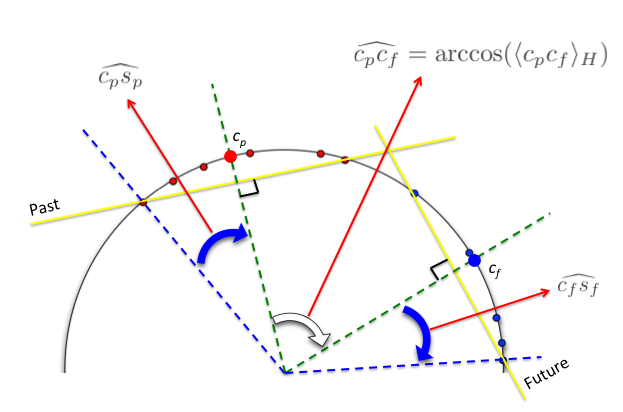
\includegraphics[width=0.5\textwidth]{kcd.png}
\caption{KCD Geometry in Feature Space}
\label{fig:kcdGeo}
\end{center}
\end{figure}

\begin{equation}
\label{eq:kcd}
KCD_{stat} = \frac{\widehat{c_pc_f}}{\widehat{c_fs_f} + \widehat{c_ps_p}}
\end{equation}

These angles can be calculated using the inverse cosine of the dot product between the weight vectors, as shown in Eq. \ref{eq:kcd2}.
One should note the denominator in Eq. \ref{eq:kcd2} is for normalizing the vectors to unit length.
This normalized dot product can be calculated in input space using SVM's learned weights $\boldsymbol{\alpha_p}$ and $\boldsymbol{\alpha_f}$ and the kernel matrices $K$ as shown in Eq. \ref{eq:kcd3}.
To obtain the within-class spread for each class, we use a similar form but rely on the SVM's intercept $\rho$ rather than a dot product, as shown in Eq. \ref{eq:kcd4}.

\begin{equation}
\label{eq:kcd2}
\widehat{c_pc_f} = \arccos \left(\frac{\langle w_p, w_f \rangle_F}{\| w_p \|\| w_f \|} \right)
\end{equation}

\begin{equation}
\label{eq:kcd3}
\frac{\langle w_p, w_f \rangle_F}{\| w_p \|\| w_f \|}  = \frac{\boldsymbol{\alpha}_p^T K_{p, f} \boldsymbol{\alpha}_f }{\sqrt{\boldsymbol{\alpha}_p^T K_{p, p} \boldsymbol{\alpha}_p }\sqrt{\boldsymbol{\alpha}_f^T K_{f, f} \boldsymbol{\alpha}_f }}
\end{equation}

\begin{equation}
\label{eq:kcd4}
\widehat{c_is_i} = \arccos \left(\frac{\rho_i}{\sqrt{\boldsymbol{\alpha}_i^T K_{i,i} \boldsymbol{\alpha}_i }} \right), i \in \{ p, f \}
\end{equation}

\subsubsection{Algorithm}

KCD has four parameters: 

\begin{itemize}
\item $m$ -- Window size, or the number of points on either side of a candidate change point.
\item $\gamma$ -- SVM parameter governing bandwidth for the RBF kernel (other kernels are possible, but we did not experiment with them).
\item $\nu$ -- One-class SVM parameter governing proportion of points that should be counted as outliers when training.
\item $\eta$ -- Threshold parameter such that, if $KCD_{stat} \ge \eta$ for some time point $h$, $h$ is considered a change point.
\end{itemize}

We assume $X$ is the input data of size $n \times k$.

\begin{function}
	\SetAlgoLined
	$n \gets$ len$(X)$ \;
	\BlankLine
	changePoints $\gets [ \; ]$ \;
	\For{$h \in [m, n-m-1]$}{
		$X_{p} \gets X[h-m, h]$ \;
		$X_{f} \gets X[h, h+m]$ \;
		\BlankLine
		svm$_p \gets$ SVM.fit($X_{p}, \gamma, \nu$) \;
		svm$_f \gets$ SVM.fit($X_{f}, \gamma, \nu$) \;
		\BlankLine
		$\boldsymbol{\alpha}_p \gets \text{svm}_p.\alpha$ \;
		$\boldsymbol{\alpha}_f \gets \text{svm}_f.\alpha$ \;
		\BlankLine
		$\boldsymbol{\rho}_p \gets \text{svm}_p.\rho$ \;
		$\boldsymbol{\rho}_f \gets \text{svm}_f.\rho$ \;
		\BlankLine
		$K_{p, p} \gets \text{rbf}(X_p, X_p)$ \;
		$K_{f, f} \gets \text{rbf}(X_f, X_f)$ \;
		$K_{p, f} \gets \text{rbf}(X_p, X_f)$ \;
		\BlankLine
		$\widehat{c_pc_f} \gets \arccos \left(  \frac{\boldsymbol{\alpha}_p^T K_{p, f} \boldsymbol{\alpha}_f }{\sqrt{\boldsymbol{\alpha}_p^T K_{p, p} \boldsymbol{\alpha}_p }\sqrt{\boldsymbol{\alpha}_f^T K_{f, f} \boldsymbol{\alpha}_f }} \right)$ \;
		$\widehat{c_ps_p} \gets \arccos \left(  \frac{ |\boldsymbol{\rho}_p|}{\sqrt{\boldsymbol{\alpha}_p^T K_{p, p} \boldsymbol{\alpha}_p }} \right)$ \;
		$\widehat{c_fs_f} \gets \arccos \left(  \frac{ |\boldsymbol{\rho}_f|}{\sqrt{\boldsymbol{\alpha}_f^T K_{f, f} \boldsymbol{\alpha}_f }} \right)$ \;
		\BlankLine
		$KCD_{stat} \gets \frac{c_pc_f}{c_ps_p + c_fs_f}$ \;
		\If{$KCD_{stat} > \eta$}{
			changePoints += $h$
		}
	}
	\BlankLine
	return changePoints
 \caption{KCD($X, m, \gamma, \nu, \eta$) Algorithm by Desobry et al.\cite{1468491}}
\end{function}

\section{Performance Comparison}

\todo[inline]{Graphs}

\section{Conclusions}

\todo[inline]{Conclusions}


% use section* for acknowledgement
\section*{Acknowledgment}
This work made use of the Open Science Data Cloud (OSDC) which is an Open
Cloud Consortium (OCC)-sponsored project. The OSDC is supported in part by
grants from Gordon and Betty Moore Foundation and the National Science 
Foundation and major contributions from OCC members like the University of 
Chicago.  \todo[inline]{Insert PIRE fellow name} was supported by the 
National Science Foundation Partnerships for Research and Education (PIRE) 
Award Number 1129076. Any opinions, findings, and conclusions or 
recommendations expressed are those of the author(s) and do not necessarily 
reflect the views of the National Science Foundation. 

Make sure at some point in the paper to cite the main Open Science Data Cloud paper \cite{Grossman2012}.

% references section

% can use a bibliography generated by BibTeX as a .bbl file
% BibTeX documentation can be easily obtained at:
% http://www.ctan.org/tex-archive/biblio/bibtex/contrib/doc/
% The IEEEtran BibTeX style support page is at:
% http://www.michaelshell.org/tex/ieeetran/bibtex/
% argument is your BibTeX string definitions and bibliography database(s)
\bibliography{sources}
\bibliographystyle{IEEEtran}


\end{document}
%%%%%%%%%%%%%%%%%%%%%%%%%%%%%%%%%%%%%%%%%%%%%%%%%%%%%%%%%%%%%%%%%%%%%%%
%% STUFF FROM THE TOP
%% bare_conf.tex
%% V1.3
%% 2007/01/11
%% by Michael Shell
%% See:
%% http://www.michaelshell.org/
%% for current contact information.
%%
%% This is a skeleton file demonstrating the use of IEEEtran.cls
%% (requires IEEEtran.cls version 1.7 or later) with an IEEE conference paper.
%%
%% Support sites:
%% http://www.michaelshell.org/tex/ieeetran/
%% http://www.ctan.org/tex-archive/macros/latex/contrib/IEEEtran/
%% and
%% http://www.ieee.org/

%%*************************************************************************
%% Legal Notice:
%% This code is offered as-is without any warranty either expressed or
%% implied; without even the implied warranty of MERCHANTABILITY or
%% FITNESS FOR A PARTICULAR PURPOSE! 
%% User assumes all risk.
%% In no event shall IEEE or any contributor to this code be liable for
%% any damages or losses, including, but not limited to, incidental,
%% consequential, or any other damages, resulting from the use or misuse
%% of any information contained here.
%%
%% All comments are the opinions of their respective authors and are not
%% necessarily endorsed by the IEEE.
%%
%% This work is distributed under the LaTeX Project Public License (LPPL)
%% ( http://www.latex-project.org/ ) version 1.3, and may be freely used,
%% distributed and modified. A copy of the LPPL, version 1.3, is included
%% in the base LaTeX documentation of all distributions of LaTeX released
%% 2003/12/01 or later.
%% Retain all contribution notices and credits.
%% ** Modified files should be clearly indicated as such, including  **
%% ** renaming them and changing author support contact information. **
%%
%% File list of work: IEEEtran.cls, IEEEtran_HOWTO.pdf, bare_adv.tex,
%%                    bare_conf.tex, bare_jrnl.tex, bare_jrnl_compsoc.tex
%%*************************************************************************
